\section{Verification}
\label{Verification}
%section including all the simulation results created
Verification in matlab involved running many sweep tests of all possible signal amplitudes and DC levels.
These tests were also run with non-ideal parameters set within the model to simulate a real circuit implementation.

    \subsection{DC Stability}
    \label{Verification:DCstab}
    %tests showing DC stability with different problems
    Tones at the output of a modulator will degrade the SQNR performance of a circuit during normal operation.
    Also, the effects of DC inputs on the stability of the loop must also be investigated to find the input range of the modulator over which it is stable. 
    The effect on output DC response from an input DC sweep due to finite amplifier gain is another important factor.
    The transient output of this modulator was inspected for various input voltages and found to be stable.

    %should have a plot of just the transient voltages at different points in the circuit for high input voltages to show nothing is becoming linear
    %GET RID OF THIS IF ITS DIFFICULT TO SOURCE THE WAVE
%    \begin{figure}
%        \begin{center}
%        \includegraphics[width=0.8\textwidth]{tranexample}
%        \label{fig:tranexample}
%        \caption{An example transient output waveform.}
%        \end{center}
%    \end{figure}


        \subsubsection{DC input voltage - DC output voltage}
        \label{Verification:DCinputoutput}
        %point out how this design's dead zone performance is better than for other designs
        %so it can be implemented using amplifiers with lower gain
        The effect of finite gain amplifiers on a design can be to cause ``dead zones'' to appear in the transfer function of DC input to DC output.
        This design is expected to be resistant to this effect as it is effectively a third order design and the width of the dead zone can be expected to be proportional to $\frac{1}{A^{3}}$.

        %there is no spec for this so could just drive it down very low
        The results of this design to this test are shown in figure \ref{fig:dcdc}.
        No dead zones are visible at any zoom level - the dead zones produced are smaller than the resolution of the sweep.
        This suggests it is likely the non-linearity will not affect the design.

        \begin{figure}[hb]
            \begin{center}
            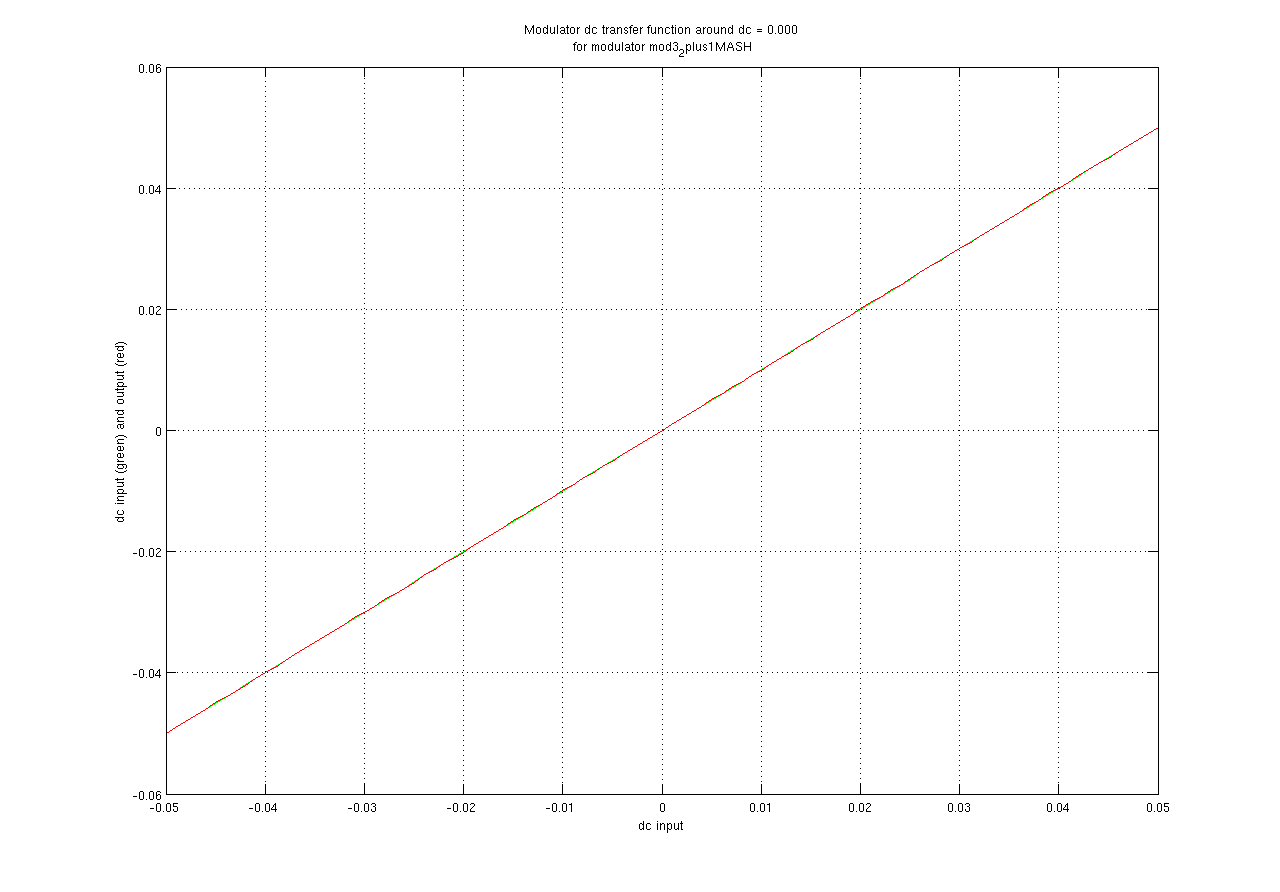
\includegraphics[width=0.8\textwidth]{dcdcMASH.png}
            \caption{DC input voltage to DC output voltage for a finite gain of 1000.} 
            \label{fig:dcdc}
            \end{center}
        \end{figure}       

        \subsection{DC input voltage - baseband power}
        \label{Verification:DCbbpwr}
        %
        A sweep of DC input voltages while monitoring the baseband power will detect tones appearing at those input voltages.
        The result of this test is shown in figure \ref{fig:dcdcbbpwr}.
        This was run with saturation limits in both integrators equal to 2.546V, to reflect the signal range required of the real circuits.

         \begin{figure}
            \begin{center}
            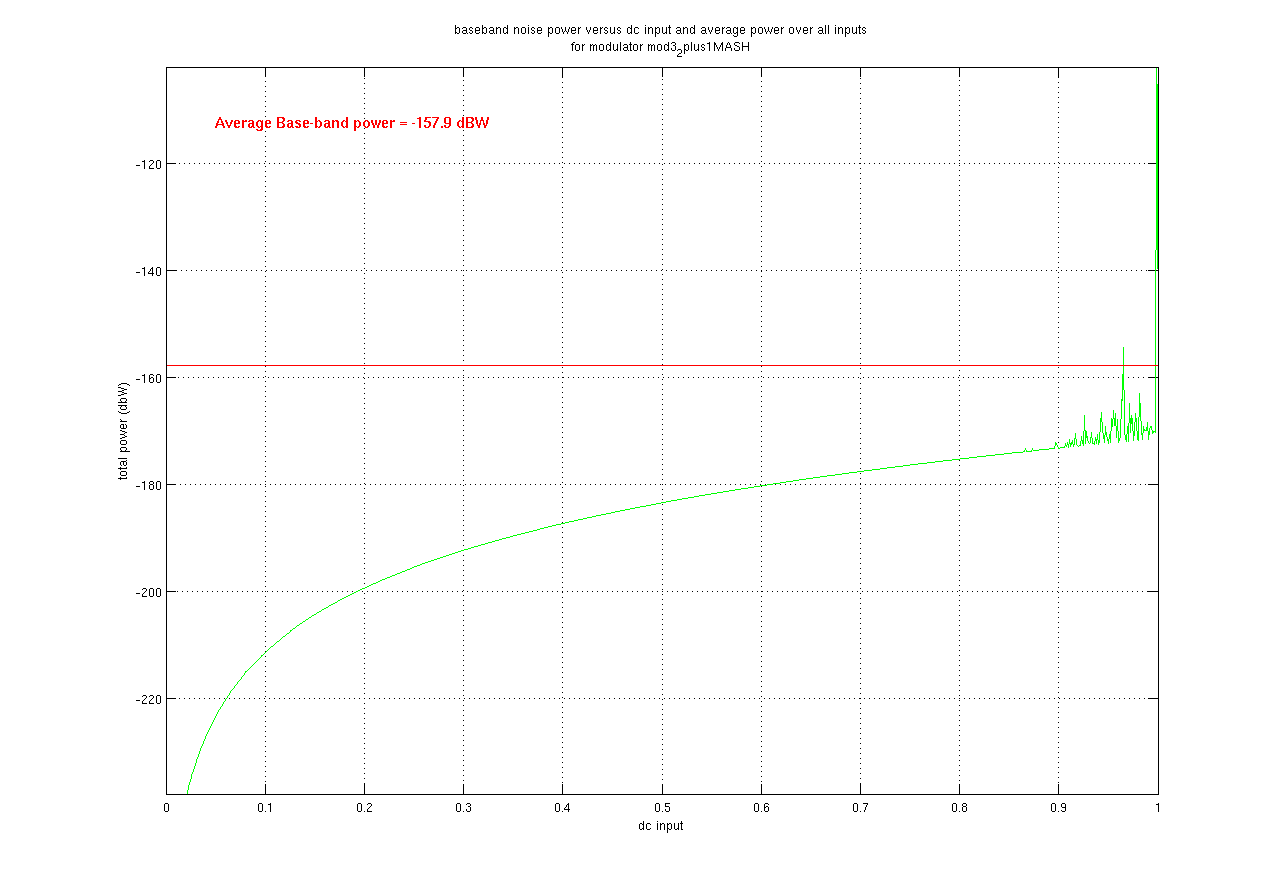
\includegraphics[width=0.8\textwidth]{dcbbpwrsweep.png}
            \caption{Nominal baseband power resulting from a sweep of DC inputs.}
            \label{fig:dcdcbbpwr}
            \end{center}
        \end{figure}       
        
        %this might result in requiring dither
        The baseband power never exceeds -103dB, so it can be expected that the circuit is well within specification.

        %investigate the effect of mismatch?

%    \subsection{Flat Noise Profile}
%    %using dither to make the noise profile flat
%    The noise profile of the chosen design without dither can be seen in figure \ref{fig:MASH}.
%    It does not meet the specifications in that it is not flat.
%    This is a problem that can be solved by applying dither to the circuit in the form of adding random noise at 
%
%    \begin{figure}
%        \begin{center}
%        \includegraphics[width=0.8\textwidth]{SQNRdither}
%        \label{fig:SQNRdither}
%        \caption{Single simulation showing the effect of dither on the noise floor of the modulator.}
%        \end{center}
%    \end{figure}  
%
%    Dither is therefore applied in all SQNR simulations involving this modulator.

    \subsection{SQNR Stability}
    %sweeps of SQNR
    To verify the performance of a Sigma-Delta modulator it is necessary to verify the resolution of the circuit at many input amplitudes and in cases involving non-ideal components.
    The cases tested here are:
    \begin{itemize}
        \item Capacitor mismatch
        \item Finite gain
        \item Stage mismatch
        \item Finite signal swing
    \end{itemize}

    Without mismatch, but with a finite gain of 1000 and a finite signal swing equal to that expected in the amplifier of 2.546V differential, the results of a sweep of input sine amplitudes is shown in figure \ref{fig:SQNRnominal}.

    \begin{figure}
        \begin{center}
        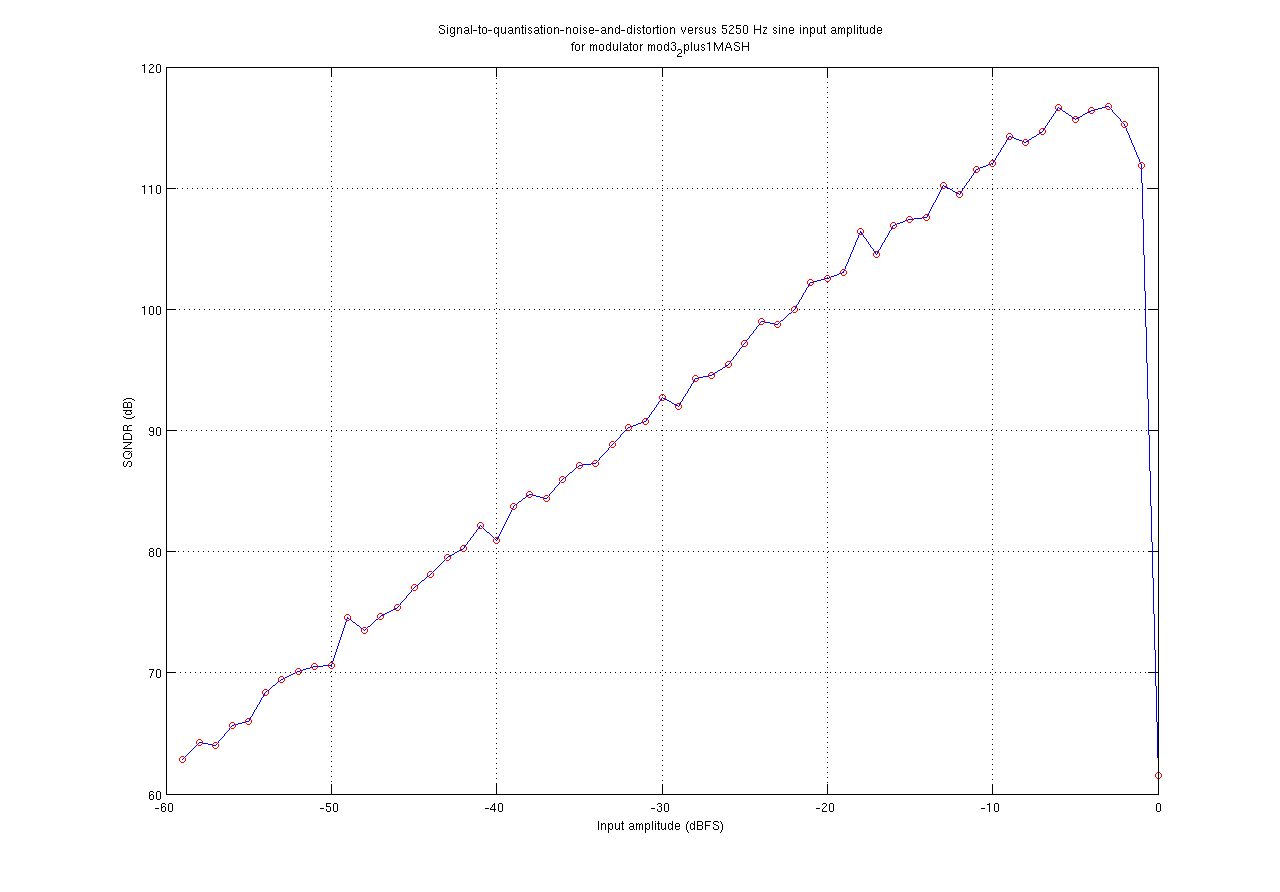
\includegraphics[width=0.8\textwidth]{MASHSQNRsweep0105.png}
        \caption{SQNR resulting from a sweep of different input amplitudes of a sine wave without mismatch is shown.}
        \label{fig:SQNRnominal}
        \end{center}
    \end{figure}  



        \subsubsection{Capacitor Mismatch}
        %capacitor mismatch, the effect of
        Capacitor mismatch causes a mismatch in the multiplication stages of the amplifier.
        In the matlab model there are various precise multiplication elements that can be varied.
        The variation expected in capacitors is 0.4\%, so a variation in these values of 0.4\% must be tested.
        For a design margin, this can be increased to 1\% mismatch on the two gains to modify in the design, shown in figure \ref{fig:MASH}.

        Applying gain mismatch of 1\% in all four possible configurations; the worst observed result is shown in figure \ref{fig:SQNRcap} - swept for all input amplitudes.
        The worst observed was a combination of 99\% mgain2 and 101\% mgain1.
        Figure \ref{fig:SQNRcap} shows that the circuit is still able to meet the specification.
 
        \begin{figure}
            \begin{center}
            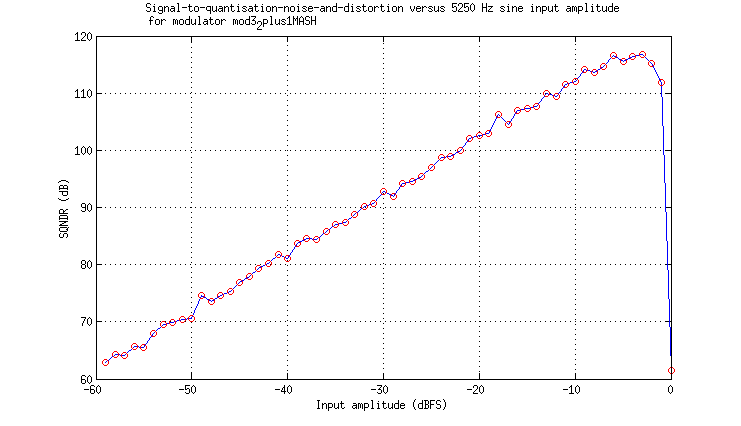
\includegraphics[width=0.8\textwidth]{MASHsweepcap.png}
            \caption{SQNR resulting from a sweep of different input amplitudes of a sine wave with capacitor mismatch is shown.}
            \label{fig:SQNRcap}
            \end{center}
        \end{figure} 

        \subsubsection{Effect of Noise Leakage} 
        \label{Verification:leakage}
        %run SQNR sweeps with mismatches in the transfer function
        %reference equations describing this from the textbook
        Noise leakage is governed by the mismatch of transfer functions from the fist and second stages of the modulator(\cite{Schreier2004}, p.132).
        This requires modifying gain components defining the individual stages.
        With the worst case gains from the previous section set, these two internal gain blocks were modified by 1\% mismatch to find the worst combination.
        The result is shown in a sweep of all input amplitudes in figure \ref{fig:SQNRtrans}.

        \begin{figure}
            \begin{center}
            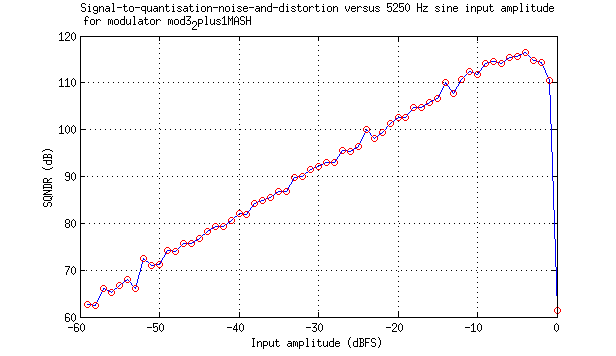
\includegraphics[width=0.8\textwidth]{MASHsweeptrans.png}
            \caption{SQNR resulting from a sweep of different input amplitudes of a sine wave with transfer function mismatch is shown.}
            \label{fig:SQNRtrans}
            \end{center}
        \end{figure} 

    \subsection{Cadence Tests}
    %test showing that the sizing of switches and caps is ok
    To show that the sizing of devices in section \ref{Design:components} is correct, the modulator should be simulated to show that the input referred noise is as low as expected.
    Unfortunately, the full modulator was not implemented in Cadence, making this full simulation impossible.
    To prove that the sizing is adequate a first order modulator noise simulation was performed with the input capacitor and $g_{m}$ sizing calculated applied.

    %notes on resizing to meet specification
    First order calculations proved to be inaccurate at this point and it was necessary to further increase the size of the input capacitors to meet the noise requirements.
    It was also necessary to increase the amplifier input $g_{m}$, output $g_{m}$ was also scaled approximately in anticipation of the effect of higher capacitance on settling requirements - although, settling was not tested.
    The final values producing the noise results seen in Appendix \ref{Appendices:noise} can be seen in table \ref{tab:finalsizing}.

    \begin{table}
    \begin{center}
    \caption{The final capacitor and $g_{m}$ sizings found through simulation of a first order modulator.}
    \label{tab:finalsizing}
    \begin{tabular}{l p{0.15\textwidth}} 
    \toprule
    Component  & Value \\
    \midrule
    input $g_{m}$ & $500\mu A/V$ \\
    output $g_{m}$ & $500\mu A/V$ \\
    input $R_{ds}$ & $2M\Omega$ \\
    output $R_{ds}$ & $20k\Omega$ \\
    $C_{in}$ and $C_{fbk}$ & $8pF$ \\
    \end{tabular}
    \end{center}
\end{table}


    %estimate the SQNR that would be achieved by adding worst case quantisation noise and worst case thermal noise
    The final thermal noise power achieved is therefore $10.2\mu V$, this can be combined with the worst case expected SQNR to create an estimate of SNDR for this design.
    Worst case SNDR was observed in section \ref{Verification:leakage} was 116.9dB, this equates to $2.57\mu V$ RMS noise.
    Combining these in quadrature yields $10.52\mu V$ and an effective SNDR of 104.7dB SNDR.


\subsection{Conclusion}
\label{Verification:conclusion}
%conclusion to the verification section
Although a full simulation of a macro-model implementation of the modulator has not been completed, the simulation results presented here show that this circuit is capable of meeting the specifications as described.
Non-ideal effects have been considered in the matlab simulations and noise has been investigated in the Cadence simulations.
From these results the circuit can be expected to work if completed.

